\chapter{Modelos de comportamiento}
\label{ch:sota-behavior-models}

El objetivo que persigue la simulación de tráfico es hacer cada vez más realistas los modelos generados. Cuando el simulador está basado en \glsentrylongplsp{mas}, el realismo aumenta cuanto más se parece el comportamiento de los agentes al de los conductores reales.

Conducir implica la ejecución de múltiples tareas en paralelo, cada una de ellas pertenecientes a un nivel cognitivo. Además, las acciones no están limitadas a la interacción con el vehículo; el conductor ha de tener en cuenta otros factores como, por ejemplo las señales, los peatones o los \glspl{adas}.

\begin{figure}
	\centering
	\begin{tikzpicture}
	\tikzset{
		centered/.style = { align=center, anchor=center },
		arrow/.style = { black!20, arrows={-Triangle} },
		dblarrow/.style = { black!20, arrows={Triangle-Triangle} },
	}
	
	\matrix (m) [
	matrix of nodes,
	column sep      = 2em,
	row sep         = 1em,
	column 1/.style = { nodes = { font=\sffamily\scriptsize, fill=black!20, centered}},
	column 2/.style = { nodes = { font=\sffamily, centered, fill=orange!20, text width=3cm }},
	column 3/.style = { nodes = { font=\sffamily, centered, text width=2.2cm }},
	column 4/.style = { nodes = { font=\sffamily, centered }},
	] {
		& Nivel estratégico & planes generales & $\gg s.$\\
		Entorno & Nivel táctico  & patrones de acción & $s.$ \\
		Entorno  & Nivel de control & comportamientos automáticos & $ms.$ \\
	};
	\draw[arrow] (m-1-2) -> (m-1-3);
	\draw[arrow] (m-2-1) -> (m-2-2);
	\draw[dblarrow] (m-2-2) -> (m-2-3);
	\draw[arrow] (m-3-1) -> (m-3-2);
	\draw[dblarrow] (m-3-2) -> (m-3-3);
	\draw[dblarrow] (m-2-2) -> (m-1-2);
	\draw[dblarrow] (m-3-2) -> (m-2-2);
	\end{tikzpicture}
	\caption{Los tres niveles jerárquicos que describen la tarea de conducción según~\cite{michon1985critical}: \textit{estrategia} (i.e. las decisiones generales), la \textit{maniobra} (i.e. decisiones durante la conducción de más corto plazo) y \textit{control} (i.e. automatismos).\TODO{Esta ilustración es una puta mierda. Tiene que ser más bonita, por dios!}}
	\label{fig:three-levels-of-human-driving}
\end{figure}

\cite{michon1985critical} divide en tres los niveles de abstracción de las tareas: el de \textbf{control}, que se ocupa de las tareas de más bajo nivel como son el mantenimiento de la velocidad o los cambios de marcha, el de \textbf{maniobra} o táctico, donde sus tareas son las encargadas de mantener la interacción con el entorno como los cambios de carril o el control de las señales y demás estímulos externos, y el \textbf{estratégico}, que engloba las tareas de más alto nivel como el razonamiento y la planificación de rutas (ver figura~\ref{fig:three-levels-of-human-driving})\sidenote{Algunos estudios llegan incluso a definir intervalos temporales de tiempo de razonamiento para las tareas de cada nivel. Por ejemplo, en \cite{Alexiadis2004} se establecen los siguientes tiempos: alrededor de $30$ segundos para las tareas del nivel de planificación, de $5$ a $30$ segundos para las tareas de nivel táctico y por debajo de los $5$ segundos para las tareas de control.}.

Otro modelo jerárquico de tres niveles muy referenciado en la literatura es el \textit{skill-rule-knowledge} de \cite{Rasmussen1986}, el cual no es más que una pequeña generalización del modelo propuesto por \cite{michon1985critical} al comportamiento y razonamiento humano. Postula que éste se puede basar en \textbf{habilidades} (actividades completamente automatizadas de la forma \textit{percepción $\rightarrow$ ejecución}), en \textbf{reglas} (situaciones familiares o estereotipadas de la forma \textit{percepción $\rightarrow$ reconocimiento de la situación $\rightarrow$ planificación $\rightarrow$ ejecución}) y en \textbf{conocimiento} (actividades conscientes que implican resolución de problemas y toma de decisiones de la forma \textit{percepción $\rightarrow$ reconocimiento de la situación $\rightarrow$ toma de decisión $\rightarrow$ planificación de la ejecución}) que suelen ser necesarias en situaciones poco familiares)\sidenote{
	El framework desarrollado en \cite{Chaib-draa1994} se basa en esta jerarquización del razonamiento humano y abarca los $3$ niveles de abstracción representando en un escenario urbano tres tipos diferentes de situaciones: rutinaria, familiar y no familiar.
}.

El comportamiento de un conductor al volante tiene una relación directa con el nivel de abstracción táctico. Se puede entender como el encargado de planificar acciones a corto plazo para conseguir objetivos a corto plazo. Las tareas de control son automáticas e influyen poco o nada en las tomas de decisión relacionadas con tareas del estilo de cuánto acelerar en esta situación o cuándo cambiar de carril. Las tareas estratégicas estan a un nivel más alto de abstracción (e.g. la ruta a seguir hasta mi destino) y tampoco afectan demasiado al comportamiento en situaciones concretas\sidenote{
	No obstante algunos trabajos han demostrado que en ocasiones la planificación de la ruta sí afecta a decisiones normalmente asociadas el nivel táctico como por ejemplo la preferencia de un conductor por uno u otro carril de la vía \cite{Wei2000, Toledo2003}.
}.

\newthought{Nuestro interés es el uso de agentes} como unidades en simulación. Después de todo trabajamos con \glspl{mas}. Sin embargo, y aunque en los trabajos más modernos exista una cierta desviación hacia este paradigma, no todos los trabajos se basan en éste. El auge de su uso coincide con el renacimiento de la \glsentrylongsp{ai}, alrededor de los años $90$, y los modelos que se describen en este apartado, sobre todo posteriores a esta fecha, se basan en este tipo de sistemas.

Las tipologías de agentes utilizadas es de tido tipo. Existen desde trabajos que explotan las características de los agentes reactivos (e.g. en \cite{Ehlert2001} se estudian agentes que continuamente van realizando decisiones de control para mantenerse en la via y llegar a su destino) hasta aquellos que proponen frameworks nuevos para definir comportamientos\sidenote{
	Un \textit{framework} muy interesante de modelización de comportamiento de conductores es el propuesto por \cite{al2001framework}. Éste se basa en cuatro unidades de funcionamiento interconectadas, la de \textbf{percepción}, que percibe el entorno en términos locales y globales, la de \textbf{emoción}, que se ocupa de identificar cómo responde emocionalmente al entorno, la de \textbf{toma de decisiones}, que investiga posibles acciones que podrían servir a las necesidades del módulo emocional y la de \textbf{ejecución de decisiones}, que intenta implementar las decisiones cuando emergen condiciones de tráfico lo suficientemente seguras para llevarlas a cabo. \TODO{poner ilustración y volver a leerlo para incluir conclusiones. No parece que sean nada del otro mundo más allá que agentes basados en utilidad, pero bueno. Más allá de simlpes, definen una forma de trabajar que probablemente usen el resto de frameworks y que podemos basarnos en ella.}.
}.

La información que manejan estos agentes dentro de los simuladores suele limitarse a tipologías (e.g. utilitarios o vehículos de grandes dimensiones) y magnitudes físicas (tamaño, velocidad máxima). Dependiendo del trabajo, algunos autores añaden más conocimiento a los agentes; por ejemplo, en \cite{hidas2002}, el autor incluye en los agentes, denominados \glspl{dvo} (otra forma de denominar al concepto de \gls{dvu}), información adicional sobre el tipo de conductor y el nivel de conocimiento de la red de carreteras.

El resto del capítulo introducirá los modelos de comportamiento más conocidos y hará especial hincapié en el estado más reciente de modelos basados en técnicas de la \glsentrylong{ci}.

\section{Comportamientos modelados}

\begin{figure}
	\centering
	\begin{tikzpicture}
	\tikzset{every concept/.style={minimum size=2cm, text width=2cm}}
	\path[mindmap,concept color=MidnightBlue, text=white]
	node[concept] {modelos} [clockwise from=300]
	child[level distance=100, concept color=RoyalBlue] {
		node[concept] {aceleración} [clockwise from=30]
		child[concept color=Peach] {
			node[concept] {free-flow}
		}
		child[concept color=Peach] {
			node[concept] {car-following}
		}
	}
	child[level distance=100, concept color=RoyalBlue] {
		node[concept] {lane-changing} [clockwise from=210]
		child[concept color=Peach] {
			node[concept] {lane-selection}
		}
		child[concept color=Peach] {
			node[concept] {gap-acceptance}
		}
	};
	\end{tikzpicture}
	\caption{Las diferentes tareas para modelar el comportamiento de un conductor al volante. Están clasificadas en dos tipos, de aceleración (cómo acelera/frena en función de la situación) y de cambio de carril (cuándo y cómo cambia de carril). Estas clases están formadas por diferentes subclases de comportamiento dependiendo del problema.}
	\label{fig:behavior-model-classification}
\end{figure}

Las tareas que se realizan en el nivel táctico del comportamiento son aquellas relacionadas con circular dentro del flujo de tráfico. En la literatura, estas tareas se centran en dos clases generales de problema diferentes (figura \ref{fig:behavior-model-classification}): el de la \textbf{aceleración} y el del \textbf{cambio de carril}.

Los modelos de \textbf{aceleración} se ocupan de gestionar las alteraciones de la tasa de aceleración (positiva o negativa) en un entorno lineal como lo es un carril de tráfico.

Ahora bien, el tráfico real no está compuesto por un sólo carril, sino por varios. Los modelos de \textbf{cambio de carril} tienen como objetivo identificar cuándo el conductor desea cambiar de carril y realizar dicho cambio, ya sea porque quiere mejorar su circulación (e.g. quiere realizar un adelantamiento) o porque su ruta lo requiere (e.g. está próxima la rampa de salida que quiere tomar en una autopista).

En la literatura los modelos de aceleración han sido mucho más estudiados que los de cambio de carril, entre otras cosas por la dificultad en la captura de los datos y, por tanto, por su escasez.

El estudio del comportamiento en los cambios de carril es muy interesante debido a que tiene efectos opuestos según la carga de tráfico de la vía en la que se ejecutan. Por un lado, si la carga de tráfico es de ligera, mejora la velocidad media del flujo de la vía. Sin embargo, según aumenta la carga de tráfico, los cambios de carril comienzan a afectar a éste en formas de ondas de choque (\cite{Sasoh2002, Jin2006}) e interferir incluso más que los modelos de \textit{\idx{car-following}} (\cite{Laval2006}).

\subsection{Nomenclatura}

Para no llevar a equívocos, en la figura \ref{fig:lane-representation-with-namings} se ilustran los actores típicos en una situación de tráfico junto con los nombres y su rol. A continuación los explicamos:

\begin{figure}
	\missingfigure[figheight=4cm]{Ilustración estupenda y maravillosa de los vehículos en la vía y cómo están relacionados unos con otros.}
	\caption{Representación de los vehículos en una vía junto con la nomenclatura a usar durante el resto de la tesis.}
	\label{fig:lane-representation-with-namings}
\end{figure}

\begin{itemize}
	\item \textbf{Lag car}.
	\item \textbf{Lead car}.
\end{itemize}

\section{Modelado de conductores clásico}

Los primeros trabajos sobre modelos de conducción datan de comienzo de los años $50$ con estudios sobre el concepto denominado \textbf{\idx{car-following}}, acuñado por \cite{reuschel1950fahrzeugbewegungen}. Un vehículo está en una situación \idx{car-following} cuando su velocidad está condicionada por el vehículo que se encuentra frente a él. En el primer modelo concreto (\cite{Pipes1953}), el comportamiento responde a tratar de mantener un espacio variable en función de la velocidad.

\begin{marginfigure}
	\centering
	
	\smartdiagramset{
		border color=none,
		back arrow disabled=true,
		text width=2.5cm
	}
	\smartdiagram[flow diagram:vertical] {
		Mantenimiento de medidas,
		estímulo~/ respuesta,
		psico-físicos
	}
	\caption{Evolución de los tres tipos generales de modelo de \textit{car-following}: mantenimiento de medidas, estímulo$\rightarrow$respuesta y psico-físicos. Con la llegada de los psico-físicos se vio que \textit{car-following} no era más que uno de tantos regímenes distintos dentro de los modelos de aceleración.\TODO{Esto es un mojón de ilustración.}}
	\label{fig:car-following-there-different-models}
\end{marginfigure}

Este modelo se puede considerar de una clase que denominaremos \textbf{mantenimiento de medida} dado que su objetivo es mantener constantemente una distancia segura, determinada a partir de la ecuación de la velocidad cuando el tiempo no baja de $1,02$ segundos. Otros trabajos trabajan con el mantenimiento de otras medidas como distancia relativa al parachoque delantero o trasero.

\marginnote{
	El modelo \glsentryshort{ghr} (también conocido como modelo \gls{gm}) presentado en \cite{Chandler1958} es el modelo más conocido antes de la introducción del modelo de Gipps. Desarrollado a finales de los años $50$ dentro de la \textit{General Motors}, se caracteriza por el uso del concepto \textit{estímulo $\rightarrow$ respuesta}, donde la respuesta del vehículo (el cambio en la tasa de aceleración) es debida a la activación de un estímulo (la variación en la distancia con el vehículo delantero) tras pasar un tiempo de retardo $\tau$. Concretamente calcula el valor de la aceleración $a$ en un instante $t$ como:
	
	\begin{equation}
	a(t) = c v^m(t) \frac{\Delta v(t - \tau)}{\Delta x^l(t - \tau)}
	\label{eq:ghr-car-following-model}
	\end{equation}
	
	Siendo $t$ es el instante actual, $a(t)$ la aceleración del vehículo, $\delta v(t)$ y $\delta x(t)$ son la velocidad y distancia relativas al siguiente coche respectivamente, $v$ la velocidad del vehículo y $c$, $m$, $l$ y $\tau$ constantes, siendo ésta última el tiempo de reacción del conductor.
}

Más adelante, a finales de la decada se presentó el modelo \gls{ghr} (ver ecuación~\ref{eq:ghr-car-following-model}), el cual sirvió como base para el desarrollo de muchos modelos posteriores. Eset modelo dio origen a a una nueva clase de modelos de conducción, los de tipo \textbf{estímulo $\rightarrow$ respuesta}. 

En realidad los modelos estímulo $\rightarrow$ respuesta son la evolución lógica de los modelos anteriores, donde se pasa de un cálculo de velocidad en función de la distancia (u otra medida) a un sistema de control donde la variable a controlar es la aceleración en función de uno o varios estímulos de entrada, además con un retardo simulando el tiempo de reacción. Algunas modificaciones sobre el algoritmo original son, entre otras, la asimetría en la tasa de cambio de aceleración y deceleración (\cite{Gazis1959}) o la inclusión de segundos coches delanteros (\cite{Bexelius1968}).

Los métodos de estas dos clases tienen un problema principal: suponen que el conductor es capaz de percibir incluso el más ínfimo cambio en las variables observadas cuando la realidad no es así. Por ello, a mediados de los años $70$ apareció una nueva clase de modelos de \textit{\idx{car-following}}, denominados posteriormente como \textbf{psicofísicos} (\cite{wiedemann1974simulation}, donde se introduce el concepto de \textit{umbral perceptual} como solución a dicha limitación. El \textit{umbral perceptual} de una medida es el límite a partir del cual se percibe un cambio en dicha medida. Mediante el uso de umbrales perceptuales, se limitan las acciones de los coches a cambios perceptibles en los coches delanteros.

\begin{figure}
	\centering
	\smartdiagramset{
		set color list={
			orange!60,
			green!50!lime!60,
			magenta!60,
			blue!50!cyan
		},
		uniform connection color=true
	}
	\smartdiagram[bubble diagram]{
		modelos de\\ aceleración, free-flow, approaching, car-following, emergency
	}
	\caption{Tras la aparición de los modelos psico-físicos se comprobó que los umbrales en las percepciones y por tanto el comportamiento podía variar dependiendo de las situaciones. Por ello, el \textit{car-following} no era más que una entre diferentes clases o regímenes de aceleración. Algunos de los regímenes más usados en la literatura son \textit{free-flow}, \textit{car-following}, \textit{approaching}, y \textit{emergency}, aunque algunos autores definen nuevos regímenes, cada uno con sus límites de aplicación.}
	\label{fig:acceleration-model-classes}
\end{figure}

A finales de la década, en $1978$, se cumplió otro hito en el desarrollo de modelos de conducción. Sparmann en \cite{Sparmann1978} define el primer modelo de cambio de carril, inspirándose en las clases de modelo psicofísico. El verdadero interés de este modelo es que sentó las bases de dos conceptos que perduran hoy en día. El primero, la diferenciación entre cambio a carriles rápidos y lentos\sidenote{
	En \cite{Sparmann1978} el autor entiende la derecha como el carril lento y la izquierda como el carril rápido, y es como se entiende dentro del contexto de esta tesis. Sin embargo en otros países esta correspondencia es al revés.
}. El segundo, la diferenciación entre la selección de carril o \textit{\idx{lane-selection}} y la ejecución del cambio o \textit{\idx{merging}}.

\newthought{La viabilidad en un cambio de carril} se determina haciendo uso de modelos denominados \textit{\idx{gap acceptance}}, donde los vehículos calculan si caben o no en un determinado hueco y actuan en consecuencia.

En su origen los modelos de \textit{\idx{gap acceptance}} se desarrollaron para resolver situaciones en intersecciones e incorporaciones. En la actualidad son los modelos que se usan en el momento de después de seleccionar el cambio de carril y antes de ejecutar físicamente el cambio, y dependiendo del autor del modelo, lo incluye dentro de la operación \textit{\idx{lane-selection}} y la ejecución del cambio o \textbf{\idx{merging}}.

En general se basan en una fórmula que determina si, en función de una serie de parámetros entre los que se incluye el hueco del carril destino, el cambio es viable, en cuyo caso el cambio se ejecuta. En la ecuación~\ref{eq:gap-acceptance-model} se describe el modelo típico de un modelo de \idx{gap accceptance}. 

\marginnote{
	\paragraph{Modelo típico de \textit{\idx{gap acceptance}}}
	
	\begin{equation}
	f_{g_l}(t) = \twopartf {0} {g_l(t) < g^{crit}_l(t)} {1} {g_l(t) \geq g^{crit}_l(t)}
	\label{eq:gap-acceptance-model}
	\end{equation}
	
	En un momento $t$, el cambio a un carril $l$ es viable ($f_{g_l}(t) = 1$) o no ($f_{g_l}(t) = 0$) dependiendo de si el espacio en el carril destino $g_l(t)$ es mayor o menor que un \enquote{hueco crítico} (en inglés \idx{critical gap}) $g^{crit}_l(t)$.
}

\newthought{Llegados a este punto}, con los modelos psicofísicos se llegó a la conclusión que no todas las situaciones eran iguales, sino que en función del entorno y el momento los umbrales podían variar, y que el \textit{\idx{car-following}} no era sino un subtipo más de una clase más amplia que se definió como \textit{modelos de aceleración} (figura~\ref{fig:acceleration-model-classes}).

Debido a eso y a la irrupción de los modelos de cambio de carril, los posteriores modelos y \textit{frameworks} desarrollados se componen de dos o más submodelos que responden a diferentes umbrales. Sin embargo, esto provoca que los modelos desarrollados sean más complejos ya que, cuantos más regímenes se tratan de agrupar en un mismo modelo, más aumenta el número de factores a generalizar y ajustar.

\newthought{El trabajo de Gipps} en \cite{Gipps1981} es uno de los primeros modelos que agrupa varios regímenes distintos (concretamente \textit{\idx{car-following}} y \textit{\idx{free-flow}}). Sin embargo consideramos más interesante su posterior trabajo, \cite{Gipps1986} ya que puede considerarse como la primera solución para el cambio de carril.

\begin{figure}
	\missingfigure[figheight=4cm]{Dos ilustraciones, una con un cambio de carril obligatorio (que se acabe el carril por ejemplo) y otro discrecional (que se vea un vehículo lento como un camión y el coche adelantando).}
	\caption{Los cambios de carril se clasifican como aquellos necesarios para continuar con la conducción (obligatorios) y aquellos útiles para mejorar la situación de conducción (discrecionales).}
	\label{fig:lane-change-mandatory-vs-discretional}
\end{figure}

\marginnote{
	En el trabajo de \cite{wiedemann1992microscopic} se proponen hasta cuatro clases diferentes de modelos de aceleración en función de las posiciones y velocidades relativas entre el vehículo sujeto y el siguiente:
	
	\begin{itemize}
		\item \textbf{free-flow}. El comportamiento del vehículo no se ve afectado por el del vehículo delantero.
		\item \textbf{car-following}. El comportamiento vehículo se ve influenciado por el vehículo delantero, obligando a disminuir la velocidad deseada en el conductor en cuestión.
		\item \textbf{approaching}. Situación intermedia entre las dos anteriores
		\item \textbf{emergency}. La situación es crítica (e.g. colisión inminente) obligando, normalmente, a respuestas extremas.
	\end{itemize}
	
	Más adelante diferentes autores identifican otros regímenes que pueden considerarse en algunos casos como situaciones independientes (e.g. \textit{close-following} o \textit{stop-and-go} \cite{Toledo2003, Liu2013}).
}

Introduce el concepto de que los cambios de carril obedecen a diferentes motivaciones. Por un lado, los cambios pueden ser \textbf{obligatorios} (denominado en la literatura como \gls{mlc}) cuando los vehículos se ven obligados a abandonar el carril que ocupan. Por otro lado, pueden ser \textbf{discrecionales} cuando el cambio obedece a motivaciones más relacionadas con la mejora del confort o de la situación actual de conducción (ver figura~\ref{fig:lane-change-mandatory-vs-discretional}).

En su modelo Gipps propone un modelo para el cambio de carril al aproximarse a un cambio de dirección. Dicho modelo identifica tres distancias que caracterizan el comportamiento del conductor en función de cómo de lejos está dicho punto: (i) textbf{lejos}, en el que no existe condicionamiento en la decisión de cambio de carril, (ii) textbf{medio}, donde el conductor empieza a ignorar los cambio que dan ventaja de velocidad si no hacia carriles distanciados del de salida y (iii) \textbf{cerca} donde los vahículos deben estar en el carril de cambio de salida.

Otro concepto que incluye el modelo de Gipps y que exporta a modelos posteriores de cambio de carril\index{lane-changing} es el de ampliar el \textit{\idx{critical gap}} a más de un hueco: las distancias hasta el vehículo delantero y hasta el vehículo trasero, forzando a que durante el proceso de \idx{gap acceptance} las condiciones de ambos huecos tengan que ser aceptables.

\begin{figure}
	\missingfigure[figheight=4cm]{Tres ilustraciones, una para cada caso de lejos, medio y cerca..}
	\caption{En el modelo de Gipps, la distancia al punto determina el grado de obligatoriedad del cambio.}
	\label{fig:lane-change-type-depending-on-the-distance}
\end{figure}

Posteriormente, en \cite{wiedemann1992microscopic} se desarrolla un framework similar pero teniendo en cuenta los cambios a carriles lentos (para representar, por ejemplo, obstrucciones como accidentes o un vehículo lento) y a carriles rápidos (para situaciones como condiciones de la ruta). Además el autor incluye un modelo para influir en su desempeño en función del entorno actual (las características de los vehículos de alrededor) y el entorno potencial (la estimación de las características del entorno en momentos posteriores).

El modelo de Gipps sin embargo adolecía de dos problemas clave. Muchos de estos problemas fueron heredados por multitud de trabajos posteriores que basaban su funcionamiento o su concepto en éste.

\newthought{Un cambio de carril no sólo involucra} al conductor que lo ejecuta. El \cite{Hidas2002}, el autor resalta el problema de que, en situaciones de congestión, el cambio ha de ser o bien forzado o bien a través de colaboración; en caso contrario, los vehículos no abandonarán el carril congestionado.

Uno de los primeros trabajos en abordar el comportamiento colaborativo es el de \cite{Fritzsche1994}. En éste, se describe un modelo de microsimulación para analizar cuellos de botella (e.g. un accidente donde se bloquea uno de los carriles). Los autores describen el problema pero no consideran la modificación de los modelos en cambio de carril. \cite{Yang1996} sin embargo presenta un entorno de simulación (\gls{mitsim}) que introduce, entre otros, un modelo de cambio de carril en el que se habla específicamente de comportamiento colaborativo. Introducen el concepto de función de cortesía (\textit{\idx{courtesy yielding function}}) la cuál afecta al modelo de \textit{\idx{car-following}} de un vehículo cuando otro intenta incorporarse al carril. Sin embargo, los detalles de dicho proceso no están especificados en el artículo.

\marginnote{

}

\newthought{Además, al usar árboles secuenciales}, los factores son evaluados uno detrás de otro hasta encontrar una situación favorable, en cuyo caso el resto de factores no son evaluados. Por ejemplo, tal y como está formado el modelo de \cite{Hidas2002}, un \gls{mlc} inhibe cualquier posibilidad de realizar un \gls{dlc} independientemente de la utilidad de ambos. Para evitar esta limitación, algunos autores hacen uso de técnicas como modelos probabilísticos. Ejemplos de avances en esta línea de trabajo pueden ser \cite{Toledo2003, Toledo2007, Wei2000} (figura~\ref{fig:toledo-2007-behavior-model-tree}).

\begin{figure}
	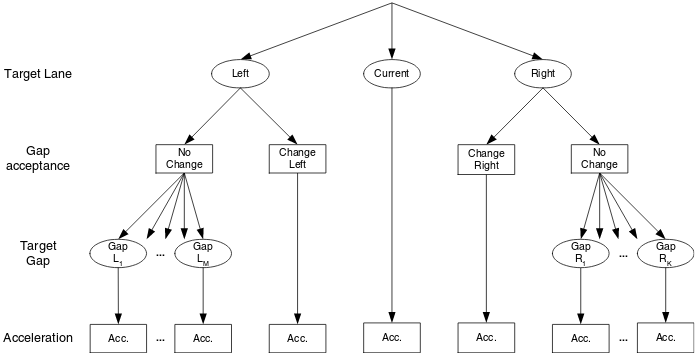
\includegraphics{toledo-2007-behavior-model-tree}
	\caption{Estructura del modelo de comportamiento de los vehículos propuesto por \cite{Toledo2007}. Este modelo se basa en el concepto de \enquote{objetivo a corto plazo} para elaborar un \enquote{plan a corto plazo} apoyándose, para ello, en un arbol de decisión. Aunque mantiene la clasificación, es probabilístico y existe opción de realizar un \gls{dlc} en lugar de un \gls{mlc} aún en situaciones donde acciones de ambas clases se activen. Clasifica las entradas en cuatro grupos de variables: las de vecindad (e.g. huecos y velocidades), las de planificación de ruta (e.g. distancia a la salida objetivo), las relacionadas con la experiencia (e.g. evitar un determinado carril en un determinado tramo) y las de estilo de conducción. Fuente: \cite{Toledo2007}.\TODO{Quizá la es muy grande. Hay que ver si merece más la pena ponerla en horizontal ocupando todo lo largo de la página y si es así, quitamos la fuente de la ilustración. Además es que es fea. Y además creo que la figura no refleja la eleccińo probabilística.}}
	\label{fig:toledo-2007-behavior-model-tree}
\end{figure}

\section{Modelado de conductores basado en \glsentrylong{ci}}

Desde mediados de los años $90$ empezó a crecer el interés por aplicar técnicas de \gls{ai} a los \gls{its}. Hay razones principales por las que esto es así: la primera, en los éxitos cosechados por la rama de la \gls{ci}, los cuales atrayeron a investigadores de multitud de áreas incluida esta. La segunda, por el rápido desarrollo de la tecnología\sidenote{
	Cada vez es cada vez más barata, más precisa y con más funcionalidades. En la última década hemos vivido una explosión de dispositivos de todo tipo: teléfonos y relojes con GPS, acelerómetros y giroscopio, ordenadores completamente funcionales del tamaño de una moneda, sensores RADAR y LIDAR para uso amateur además de profesional y así un largo etcétera.
}, que ha posibilitado la existencia de conjuntos de datos masivos con la capacidad de explotarlos y aprender de ellos.

Algunos autores (\cite{Zhang2011}) se atreven a afirmar incluso que el futuro de las \gls{its} son las técnicas de la \gls{ci}, y que los resultados que se puedan cosechar de técnicas basadas en el desarrollo convencional de sistemas es marginal comparado con las que se obtendrán con el nuevo enfoque.

Dentro de las \gls{its}, las áreas de aplicación de la \gls{ci} se centran en los siguientes conceptos: reconocimiento de patrones, caracterización de conductores y modelado de conductores. Es necesario mencionar que aunque se trate de áreas distintas, éstas suelen retroalimentarse, y es difícil encontrar estudios que se centren en una única área sin tocar el resto (figura~\ref{fig:main-applications-of-ci-in-its}). Por ello, aunque nuestro interés pueda centrarse en el modelado de conductores, es necesario conocer el estado de las demás áreas.

\begin{figure}
	\centering
	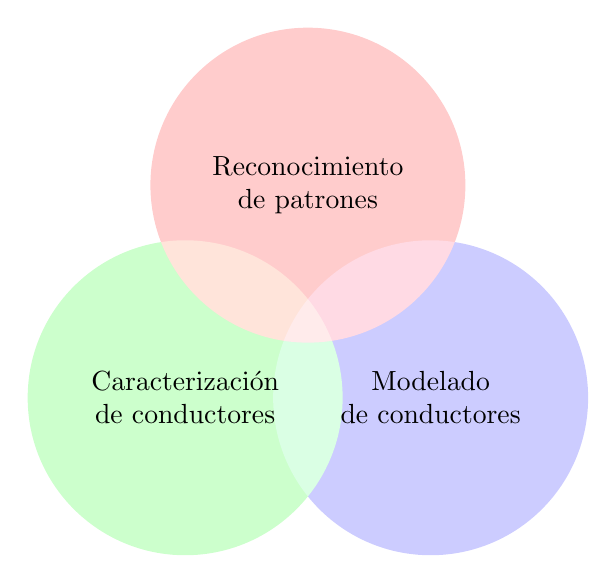
\begin{tikzpicture}
	\begin{scope}[blend group = soft light]
	\fill[red!20!white]   ( 90:1.8) circle (2);
	\fill[green!20!white] (210:1.8) circle (2);
	\fill[blue!20!white]  (330:1.8) circle (2);
	\end{scope}
	\node at ( 90:1.8) [align=center] {
		Reconocimiento\\ de patrones
	};
	\node at ( 210:1.8) [align=center] {
		Caracterización\\ de conductores
	};
	\node at ( 330:1.8) [align=center] {
		Modelado\\ de conductores
	};
	\end{tikzpicture}
	\caption{Las principales areas de aplicación de la \glsentrylong{ci} en los \glsentrylong{its} son el reconocimiento de patrones, la caracterización de conductores y la modelización de los mismos. Aunque son áreas de aplicación distintas, los estudios en general tienden a solaparse. Por ejemplo, las técnicas de reconocimiento de patrones pueden usarse como forma de extracción de características para una caracterización de conductores y a su vez esta caracterización puede usarse como base para su modelado.}
	\label{fig:main-applications-of-ci-in-its}
\end{figure}

\begin{itemize}
	\item En el \textbf{reconocimiento de patrones} las técnicas suelen trabajar en los temas de extracción de características y de predicción de comportamientos. La cantidad de datos que se pueden generar en un coche es tal que el trabajo a través de información en curdo es inviable (no digamos ya cuando los datos son extraídos de una flota de vehículos).
	\item La \textbf{caracterización de conductores} es interesante debido a que permite la identificación de perfiles de conducción y su clasificación de acuerdo a indicadores extraídos de su manera de conducir.
	\item El \textbf{modelado de conductores} nos permite la reproducción de comportamientos en simulación.
\end{itemize}

Las principales técnicas de \gls{ci} utilizadas en el modelado de conductores son las \gls{fl} y las \glspl{ann}.

\newthought{Las \glsentrylongplsp{ann}} fueron el punto de entrada de la \gls{ci} en la modelización de conductores. Los perceptrones multicapa y sus nuevas técnicas de entrenamiento se habían convertido en la nueva solución universal para todo aquel problema del que se disponiesen datos.

Las \gls{ann} se han aplicado mucho sobre el campo de las \glspl{its} en general, no sólo en modelado de conductores sino en prácticamente todos los aspectos como la conducción autónoma (\cite{huval2015empirical}), la clasificación de conductores (\cite{DiazAlvarez2014}) o la predicción (\cite{Dougherty1993, chan2012neural}) entre muchos otros.

El primer trabajo de la literatura sobre la aplicación de \glspl{ann} al modelado de conductores es \cite{Fix1990}, donde los autores desarrollan un controlador para imitar el comportamiento de un conductor. El estudio partió de una fase de conducción real en el simulador de donde se extrajeron datos para posteriormente entrenar un modelo basado en un perceptrón multicapa.

\newthought{Poco después, en $1992$ la \glsentrylongsp{fl}} fue usada también para un modelo de \textit{\idx{car-following}}. Después de todo los modelos psicofísicos aparecieron debido a que la percepción del conductor no es absoluta, sino imprecisa.

Los modelos de conducción basados en \glsentrylong{fl} parten de la hipótesis de que la información que maneja el conductor a la hora de tomar decisiones proviene de un análisis no demasiado detallado de la situación que le rodea; es decir, la percepción y el comportamiento humanos son estímulos percibidos de manera aproximada. Por tanto, el resultado debe ser fruto de un proceso de razonamiento que tenga en cuenta esa imprecisión en los estímulos.

El primer trabajo documentado en \gls{fl} es \cite{Kikuchi1992} (extendido en \cite{Chakroborty1999}), donde los autores aplicaron la lógica difusa sobre un modelo de aceleración de tipo \textit{\idx{car-following}}. Utilizaron el modelo \gls{ghr} (Ecuación~\ref{eq:ghr-car-following-model}) como base y determinaron las entradas al modelo como valores de pertenencia a conjuntos difusos. Las entradas del modelo eran las distancia y velocidad relativa entre el vehículo modelado y el delantero y la variación en la aceleración del vehículo delantero. Como salida, el cambio en la tasa de aceleración sobre el vehículo modelado.

\newthought{En realidad ambos trabajos, aunque} orientados hacia el modelo de \textit{\idx{car-following}} incluían más comportamientos por el simple hecho de su naturaleza: al ser entrenados con datos de conductores reales y manejar la información con incertidumbre, aprendieron a comportarse en diferentes regímenes (e.g. \textit{\idx{free-flow}}).

\begin{figure}
	\missingfigure[figheight=4cm]{Creo que una ilustración pequeña aquí de un controlador difuso y una red neuronal quedaría genial.}
	\caption{Al trabajar con métodos como las \glsentrylongplsp{ann} o la \glsentrylongsp{fl}, la inexactitud y la incertidumbre son ciudadanos de primera clase y forman parte de los modelos solución.}
	\label{fig:ann-and-fl-work-with-uncertainty}
\end{figure}







\newthought{Existen otras técnicas} usadas en la 

En \cite{Hou2011} proponen una técnica basada en modelos ocultos de Markov para la identificación de posibles cambios de carril. Los conductores conducen vehículos en un simulador de autopistas. A partir del ángulo de giro del volante el modelo es capaz de estimar, con una precisión del $0,95$, si el conductor va a realizar un cambio a la derecha, a la izquierda o si va a mantenerse en el carril. Creo que \cite{Berndt2008} es también por el estilo. De hecho puede que el primero es haya \enquote{inspirado} mucho.
...

Otros trabajos relacionados con la influencia del entorno y en el comportamiento colaborativo son \cite{Ahmed1999}.

En \cite{Hidas2002} también se desarrolla un modelo que separa las jerarquías en situaciones de \gls{mlc} y \gls{dlc}, además de añadir más situaciones que pueden disparar un cambio de carril. Algunos trabajos en la línea de los anteriores pueden ser \cite{Yang1996, Halati1997, Ahmed1999}.


\newthought{Cooperación entre agentes}

Una de las deficiencias de los modelos vistos hasta el momento es que no capturan los comportamientos de los diferentes tipos de conductor o de vehículo. Sin embargo, el comportamiento puede variar en función de los comportamientos de los vehículos que se encuentran en su entorno (\cite{Tordeux2010}).

Algunos estudios recientes sí que los incorporan debido a que uso de modelos de la \gls{ci} como las \glsentrylongpl{ann} (e.g. \cite{Simonelli2009, Fusco2013}), que se alimentan con datos del coche y del entorno y, por tanto, llegan a aprender detalles de éstos. Entraremos más en detalle dentro de este mismo capítulo en éstas y otras técnicas de la \gls{ci}.

Los DVO aquí tienen las siguientes debilidades: no tienen memoria (sólo planean el segundo siguiente de acuerdo a la información actual) y tienen poco contacto directo con los demás DVOs de alrededor (saben del de delante y del de detrás, pero no de los lados).
...




En~\cite{sekizawa2007modeling} describen modelos supervisados offline para capturar el comportamiento del conductor basados en auto-regresión a trozos. Más adelante lo extienden en~\cite{terada2010multi}, aunque los datos de entrenamiento son extraídos directamente de simulaciones, no del \enquote{mundo real\textsuperscript{TM}}.

Otros usos de las técnicas de la \gls{ci} como la caracterización de los conductores no serán explorados. Algunos estudios de interés son \cite{sekizawa2007modeling, terada2010multi} donde se hace uso de regresión parcial sobre datos extraídos de simuladores para la caracterización del comportamiento y \cite{DiazAlvarez2014} donde se aplican redes neuronales a datos de conducción reales para la predicción del consumo y la identificación de comportamientos agresivos.
...

\newthought{modelos basados en lógica difusa}

...

En \cite{Das} se realiza una simulación de comportamiento de vehículos en autopista. Los agentes basan su comportamiento en un sistema difuso donde las reglas definen la conclusión en autopista (i.e. car-following y lane-changing). Llaman a este simulador AASIM (Autonomous Agent Simulator).,


\newthought{modelos basados en redes neuronales artificiales}

\newthought{otras técnicas y modelos mixtos}

En \cite{Kuge2000} proponen un framework de identificar comportamiento de conductor basado en modelos ocultos de Markov.

...







\subsection{Modelos de cambio de carril}

\begin{figure}
	\missingfigure[figheight=4cm]{Dos ilustraciones, una con la selección de cambio de carril y otra con el cambio.}
	\caption{El cambio de carril se divide tradicionalmente en una operación que involucra dos pasos. La selección de carril (\textit{lane-selection}) al que cambiarse y la ejecución del cambio (\textit{merging}).}
	\label{fig:lane-selection-plus-merging}
\end{figure}

Los modelos de cambio de carril o \textit{\idx{lane-change}} se ocupan de determinar cuándo y cómo se desplaza del carril origen a un carril destino. Quizá el modelo presentado por Gipps\sidenote{
	\TODO{Escribir aquí un resumen del modelo de Gipps. Hay poco sitio. Mejor, así lo hago breve que la gente secansa de las formulitas. Si da para un par de ecuaciones, un par de párrafitos y una imagen, fetén.}
} en $1986$ (\cite{Gipps1986}) es el conocido como primera solución al problema del cambio de carril.





El primero de los conceptos se mantiene prácticamente constante en la mayoría de los modelos de la literatura. Sin embargo, algunos autores añaden nuevos pasos en al diferenciación de cambio de carril, anuque en general, dichos pasos sólo obedecen a pequeñas especializaciones antes o después de los pasos originales. Por ejemplo, en \cite{Ahmed1999} el autor propone la división del primer paso (\textit{\idx{lane-selection}}) en dos: \textit{\idx{change-decision}}\sidenote{
	Este paso concreto definido en \cite{Ahmed1999} es en realidad parte del arbol de decisión probabilístico de su modelo. Dado que este modelo nicluye además un submodelo de aceleración dentro del árbol, es comprensible que quiera incluir dicho paso en el modelo de cambio de carril.
} y \textbf{\idx{lane-selection}}.

Y también algunos autores añaden sus variaciones para especializar casos concretos como en \cite{Ahmed1999}, donde se incluye el cambio \textbf{forzado} como especialización de cambio en situaciones de mucha congestión de tráfico\sidenote{
	La razón de esta especialización es el mal desempeño del modelo de Gipps en situaciones de congestión, ya que supone que el cambio de carril ocurre sin forzar a los vehículos del carril de destino a modificar su comportamiento como disminuir la velocidad o parar.
}.




(GAP ACCEPTANCE) Algunos ejemplos de factores de influencia en el modelo de \textit{\idx{gap acceptance}} son la del tipo de cambio (\gls{mlc} o \gls{dlc}, usado en \cite{Ahmed1999, Toledo2007}), la velocidad absoluta del vehículo (\cite{Gipps1986, Ahmed1996}), la relativa con los vehículos delantero y trasero del carril destino (\cite{Ahmed1999}) o incluso el peso de encontrarse o no en una situación de cooperación (\cite{Ahmed1999, Hidas2002}).


\section{La \glsentrylong{ci} en los modelos de conducción}

\newthought{La detección de patrones es un paso necesario} para la consecución de dos objetivos básicos: la identificación y la predicción.

...

\textbf{detección de patrones en general}

\cite{sekizawa2007modeling}, \cite{terada2010multi} y \cite{bando2013unsupervised}, \cite{maye2011bayesian} (online), \cite{johnson2011driving}, \cite{van2013driver} \cite{bender2015unsupervised} basan su funcionamiento (offline u online) en la detección de patrones en conjuntos de datos masivos para pasar a una extracción de características y realizar desde ahí el proceso de clasificación.

Esto es debido a que la cantidad de datos que se pueden generar en un sólo coche (no digamos ya una flota de ellos) es tan grande que para determinados sistemas disponer de información de más alto nivel haría más sencillo su desempeño (por ejemplo, \gls{adas} que funcionasen con datos de \enquote{adelantando} que sus valores de giro, aceleración en una ventana temporal).

En~\cite{satzoda2013towards}, haciendo uso de la información combinada de bus CAN, cámaras, GPS e información digitalizada el mapa donde se circula se determina una amplio abanico de información crítica en diferentes condiciones de la carretera. La información que sacan es: número de cambios de carril a la derecha, a la izquierda, tiempo en autopista y carretera urbana, distancia recorrida, velocidades medias en autopista y urbano, paradas, giros a la derecha, a la izquierda, incormporaciones y salidas de autopsta, tiempo gastado en un sólo carril, curvas a la izquierda, curvas a la derecha y distancia media al carril central

\textbf{predicción}

En \cite{Dougherty1993} usan redes para determinar el nivel de congestión en la vía.

En \cite{terroso2015complex} hacen uso de un \gls{cep} que procesa los diferentes sensores del vehículo para detectar y analizar patrones característicos con técnicas tales como clasificadores basados en \gls{fl} y, de esta manera, predecir no sólo el número de ocupantes, sino la tipología o clase de ocupante (e.g. niños, adultos, \ldots).

\newthought{La caracterización de conductores} es interesante porque permite identificar perfiles de conducción y clasificar a los conductores de acuerdo a indicadores extraídos de su manera de conducir. Por ejemplo, en \cite{van2013driver} hacen uso de datos extraídos de sensores de inercia para construir un perfil de conductor, concluyendo que frenar y girar son mejores indicadores para la caracterización que la aceleración.

En~\cite{bando2013unsupervised} describen otro modelo no supervisado offline basado en un modelo bayesiano no paramétrico para la clusterización, combinado con un LDA (Latent Dirichlet Allocation, sea lo que sea esto) para la clusterización a más alto nivel. (\TODO ¿este método usa datos reales?)

Estos trabajos (\cite{sekizawa2007modeling}, \cite{terada2010multi} y \cite{bando2013unsupervised}) tienen la desventaja de ser computacionalmente muy costosos y con poca precisión en el caso de variar mucho los escenarios de entrenamiento y de test.

En~\cite{maye2011bayesian} se presenta un modelo online donde se infiere el comportamiento del conductor haciendo uso de una IMU (Intertial Measurement Unit) y una cámara. Primero de la IMU se sacan datos que se separan en fragmentos para luego relacionarlos con las imágenes obtenidas de la cámara. (\TODO ¿Hacia dónde mira la cámara?). Los modelos propuestos en~\cite{johnson2011driving} y~\cite{van2013driver} también se apoyan en el funcionamiento de clasificar las segmentaciones de una IMU, pero con técnicas distintas y sin cámara. Además hacen uso de señales externas y umbrales de activación para hacer más efectiva la clasificación (\TODO corroborar).

En el artículo~\cite{bender2015unsupervised} se usa también un modelo no supervisado online con una aproximación bayesiana para identificar los puntos de cambio sin depender de parámetros externos (e.g. umbrales o señales). Se basa también en (1) segmentar los datos de conducción y (2) asignar estos datos a clases que se corresponde n con comportamientos de conducción. Tiene la ventaja de ser más eficiente y rubusto que los anteriores.

...

En~\cite{sekizawa2007modeling} describen modelos supervisados offline para capturar el comportamiento del conductor basados en auto-regresión a trozos. Más adelante lo extienden en~\cite{terada2010multi}, aunque los datos de entrenamiento son extraídos directamente de simulaciones, no del \enquote{mundo real\textsuperscript{TM}}.

\newthought{}

En \cite{Dia2002} Los parámetros relativos al comportamiento, es decir, los que definen características, forma de razonar, etcétera son extraídos de encuestas a conductores reales. De acuerdo a los autores, cada conductor con sus propias características su forma de razonar sus perceciones y sus objetivos se puede modelar como un agente.

\newthought{En microsimulación}, las técnicas dominantes de los modelos de conducción son las \glsentrylong{ann} y la \glsentrylong{fl}. Las primeras debido a ser una de las técnicas principales en la rama del \gls{ml}, y la segunda por ser una manera sencilla y cercana a la manera de razonar del ser humano.

...

Para el cambio de carril

Los modelos estudiados no tienen en cuenta las inconsistencias y la incertidumbre de las percepciones y decisiones de un conductor humano \cite{McDonald1997}. Dichos modelos pertenencen a la clase \glsentrylong{hc}, esto es, valores fijos, ecuaciones y reglas de la lógica convencional para representar el conocimiento, las percepciones y las decisiones de los conductores. La única manera que tienen los autores de añadir incertidumbre en los modelos es mediante la introducción de términos aleatorios.

Sin embargo, los conductores basan sus decisiones en sus percepciones y éstas, aunque imprecisas, no tienen por qué seguir una distribución aleatoria con distribución clásica (e.g. normal). Las técnicas basadas en \gls{ci} palian los inconvenientes típicos de estas técnicas al pertenencer sus técnicas a soluciones de la clase \glsentrylong{sc}.

\cite{Das2009} una nueva metodología para cambio de carril basada en lógica difusa. El simulador se denomina Autonomous Agent SIMulation Package (AASIM). La motivación es que los sistemas difusos son capaces de modelar sistemas no lineales complejos como  reglas de la forma \texttt{if \ldots then \ldots} y que además la lógica difusa es ideal para modelar la incertidumbre del mundo real y por tanto de las percepciones de los conductores. Clasifican los cambios de carril en MLC y DLC. En MLC las reglas tienen en cuenta la distancia al siguiente punto característico (e.g. una salida) (\TODO{a lo mejor en la ilustración del principuio podemos ponerle nombre aesto y así referirnos a ello en el resto del texto}) y el número de cambios de carril necesarios. En DLC deciden si cambiar o no basándose en el nivel de satisfacción del conductor y en el nivel de congestión en los carriles adjacentes.

\cite{McDonald1997, Wu2003} desarrollan otro modelo de simulación denominado Fuzzy LOgic motorWay SIMulation (FLOWSIM) con similares características donde establecen conjuntos difusos para el modelo. Dso categorías de cambio de carril, al lento (principalmente para evitar incordiar a los vehículos que se aproximan por detrás a velocidades superiores, usan dos variables, presión del vehículo trasero y satisfacción en el gap del carril destino) y al rápido (para ganar velocidad, variables: velocidad ganada con el cambio y oportunidad, es decir, seguridad y confort con el cambio).

\TODO{Aquí hay que meter el cuadro ese de las reglas difusas para ejemplo}

\TODO{Echar un vistazo a la tabla resumen}

... Puta idea

\cite{Hidas2002} --> También aquí hablan de los \glspl{dvo} (¿esto es un clon de \glspl{dvu}?. Tienen características individuales como (i) tipo de vehículo, (ii) magnitudes físicas (tamaño, velocidad máxima, ...), (iii) tipo de conduictor y (iv) nivel de conocimiento de la red (porque afecta en la elección de ruta). Tienen un objetivo, llegar del origen al destino tan rápido como puedan. Esto implica un conjunto de decisiones a hacer en intervalos periódicos durante su funcionamiento (i) selección de ruta cada vez que se entra en un nuevo tramo y (ii) cálculo de la aceleración en cada intervalo).


\subsection{Modelos basados en lógica difusa}

...

Data-driven approaches have already been used in developing a fully adaptive cruise control system (\cite{Simonelli2009, Bifulco2014})

Otros trabajos que trabajan con lógica difusa: \cite{Chakroborty2003, Das1999, Gao2008, Gonzalez-Rojo2000, Gonzalez-Rojo2002a, Hatipkarasulu2002, McDonald1997, Won2007, Zheng2005, Wu2003}). Ninguno de estos estudios considera diferentes tipologías de vehículos para el car following

Problemas:

\begin{enumerate}
	\item ¿Qué reglas usan los humanos para modelar su comportamiento? Desconocerlas implica modelos no realistas. En \cite{Wu2003} intenta suplir este problema con encuestas a conductores.
	\item Los problemas inherentes de los controladores difusos. ¿Cómo validar las funciones de pertenencia? ¿cómo determinar las reglas difusas?
\end{enumerate}

\subsection{Modelos basados en redes neuronales artificiales}

\cite{zheng2013}



\cite{Jia2003} son los primers en usar datos reales de un coche instrumentado usando el método Five-Wheel-System, que está especificado en su paper de aquella manera y que no me entero de nada. A partir de las entradas correspondientes a velocidad relativa, espacio relativo, velocidad y velocidad deseada (para ello, clasifican al conductor de agresivo, normal, conservador) determinan la aceleración/deceleración del vehículo. No lo aplican a ningún simulador, sólo que los valores se ajustan.

\cite{Panwai2007} redes neuronales usando el dataset de \cite{Manstetten1997} desarrollan una red neuronal para mantener la distancia con el siguiente vehículo. Este modelo sí se evaluó en el simulador AIMSUN, y los resultados muestran una buena correspondiencia entre los datos y la realidad. No replica sin embargo el comportamiento de frenar hasta parar o de acelerar desde parado.

\cite{Khodayari2012}


Problemas:

\begin{enumerate}
	\item Es imposible determinar por qué la red funciona como está funcionando.
	\item Los clásicos de los problemas de redes, el no aprendizaje y la especialización.
\end{enumerate}

...

En \cite{Hunt1994} desarrollan un modelo de decisión usando redes neuronales. El modelo funciona a partir de presentarle una entrada visual del entorno alrededor del vehículo que quiere cambiar de carril. Sin embargo, no considera la cooperación entre vehículos.

\cite{Simonelli2009} have applied neural networks to develop a real-time learning mode for capturing car-following behavior taking into consideration individual drivers’ characteristics. \cite{Bifulco2014} extended the work of \cite{Simonelli2009} into a framework for reproducing spacing in adaptive cruise control applications. While in this research we have used data derived from the same experiment as \cite{Simonelli2009}, the scope and level of complexity of the studies is very different. While all studies adopt a data-driven approach, in this paper the objective is to create a simple and practical methodology for speed estimation using car-following models for use in a microscopic traffic simulator.


\subsection{Aproximaciones híbridas}

\cite{Li2003, Ma2004} usan aproximaciones de fuzzy neural networks y neuro-fuzzy respectivamente. No proveen sin embargo de documentación y no se investiga la aplicación de estos modelos a microsimuladores de tráfico.

\cite{Aghabayk2013} usan el modelo de árboles lineales locales (LOLIMOT, \cite{Nelles2013}) que no deja de ser una aproximación neuro-fuzzy del comportamiento. Intenta incorporar imperfecciones perceptuales en un modelo de car following. El modelo está basado usando datasets reales y los resultados indican que se ajusta lo predicho con la realidad, pero no hay pruebas realizadas en microsimuladores.

En~\cite{Ma2004}, bajo la suposición de que el ser humano toma múltiples decisiones relacionadas basándose en su percepción (imprecisa) del entorno propone un método masado en un sistema de inferencia difusa para tomar decisiones tanto para el problema del \textit{car following} como para el del \textit{lane changing}, calibrando y ajustando dicho controlador mediante el uso de redes neuronales (aproximación Neuro-Fuzzy).

Otros~\cite{Colombaroni2013,Kesting2008,Chong2011,Abbas2011,Chong2011a,Abbas2012,Chong2013}

\section{Datos y papers que son sólo para comentar y no para meter en el análisis del estado del arte}

\cite{terroso2015complex} desarrollan una aplicación que, basada en un \gls{cep}, implementa un modelo de clusterización para identificar el número de ocupantes así como la tipología de los mismos. También implementan un identificador de diferentes tipos de itinerario (pongo esto por si hay que citarlo desde diferentes puntos).

\cite{reuschel1950} sólo vale para decir que es el primer momento que se habla de car following.

\cite{Pipes1953} sólo vale para hablar de los modelos de car-following de \enquote{mantenimiento de medida}.

